\documentclass[twoside]{book}

% Packages required by doxygen
\usepackage{fixltx2e}
\usepackage{calc}
\usepackage{doxygen}
\usepackage[export]{adjustbox} % also loads graphicx
\usepackage{graphicx}
\usepackage[utf8]{inputenc}
\usepackage{makeidx}
\usepackage{multicol}
\usepackage{multirow}
\PassOptionsToPackage{warn}{textcomp}
\usepackage{textcomp}
\usepackage[nointegrals]{wasysym}
\usepackage[table]{xcolor}

% Font selection
\usepackage[T1]{fontenc}
\usepackage[scaled=.90]{helvet}
\usepackage{courier}
\usepackage{amssymb}
\usepackage{sectsty}
\renewcommand{\familydefault}{\sfdefault}
\allsectionsfont{%
  \fontseries{bc}\selectfont%
  \color{darkgray}%
}
\renewcommand{\DoxyLabelFont}{%
  \fontseries{bc}\selectfont%
  \color{darkgray}%
}
\newcommand{\+}{\discretionary{\mbox{\scriptsize$\hookleftarrow$}}{}{}}

% Page & text layout
\usepackage{geometry}
\geometry{%
  a4paper,%
  top=2.5cm,%
  bottom=2.5cm,%
  left=2.5cm,%
  right=2.5cm%
}
\tolerance=750
\hfuzz=15pt
\hbadness=750
\setlength{\emergencystretch}{15pt}
\setlength{\parindent}{0cm}
\setlength{\parskip}{3ex plus 2ex minus 2ex}
\makeatletter
\renewcommand{\paragraph}{%
  \@startsection{paragraph}{4}{0ex}{-1.0ex}{1.0ex}{%
    \normalfont\normalsize\bfseries\SS@parafont%
  }%
}
\renewcommand{\subparagraph}{%
  \@startsection{subparagraph}{5}{0ex}{-1.0ex}{1.0ex}{%
    \normalfont\normalsize\bfseries\SS@subparafont%
  }%
}
\makeatother

% Headers & footers
\usepackage{fancyhdr}
\pagestyle{fancyplain}
\fancyhead[LE]{\fancyplain{}{\bfseries\thepage}}
\fancyhead[CE]{\fancyplain{}{}}
\fancyhead[RE]{\fancyplain{}{\bfseries\leftmark}}
\fancyhead[LO]{\fancyplain{}{\bfseries\rightmark}}
\fancyhead[CO]{\fancyplain{}{}}
\fancyhead[RO]{\fancyplain{}{\bfseries\thepage}}
\fancyfoot[LE]{\fancyplain{}{}}
\fancyfoot[CE]{\fancyplain{}{}}
\fancyfoot[RE]{\fancyplain{}{\bfseries\scriptsize Generated by Doxygen }}
\fancyfoot[LO]{\fancyplain{}{\bfseries\scriptsize Generated by Doxygen }}
\fancyfoot[CO]{\fancyplain{}{}}
\fancyfoot[RO]{\fancyplain{}{}}
\renewcommand{\footrulewidth}{0.4pt}
\renewcommand{\chaptermark}[1]{%
  \markboth{#1}{}%
}
\renewcommand{\sectionmark}[1]{%
  \markright{\thesection\ #1}%
}

% Indices & bibliography
\usepackage{natbib}
\usepackage[titles]{tocloft}
\setcounter{tocdepth}{3}
\setcounter{secnumdepth}{5}
\makeindex

% Hyperlinks (required, but should be loaded last)
\usepackage{ifpdf}
\ifpdf
  \usepackage[pdftex,pagebackref=true]{hyperref}
\else
  \usepackage[ps2pdf,pagebackref=true]{hyperref}
\fi
\hypersetup{%
  colorlinks=true,%
  linkcolor=blue,%
  citecolor=blue,%
  unicode%
}

% Custom commands
\newcommand{\clearemptydoublepage}{%
  \newpage{\pagestyle{empty}\cleardoublepage}%
}

\usepackage{caption}
\captionsetup{labelsep=space,justification=centering,font={bf},singlelinecheck=off,skip=4pt,position=top}

%===== C O N T E N T S =====

\begin{document}

% Titlepage & ToC
\hypersetup{pageanchor=false,
             bookmarksnumbered=true,
             pdfencoding=unicode
            }
\pagenumbering{alph}
\begin{titlepage}
\vspace*{7cm}
\begin{center}%
{\Large My Project }\\
\vspace*{1cm}
{\large Generated by Doxygen 1.8.13}\\
\end{center}
\end{titlepage}
\clearemptydoublepage
\pagenumbering{roman}
\tableofcontents
\clearemptydoublepage
\pagenumbering{arabic}
\hypersetup{pageanchor=true}

%--- Begin generated contents ---
\chapter{My Personal Index Page}
\label{index}\hypertarget{index}{}Use this this class to set up an obstacle \hyperlink{classObstacle}{Obstacle} class includes a function that returns the position of obstacle


\begin{DoxyParams}{Parameters}
{\em Has} & parameters radius and position\\
\hline
\end{DoxyParams}
This is a mainpage for a first doxygen file test for a robot program. 
\chapter{Todo List}
\label{todo}
\Hypertarget{todo}

\begin{DoxyRefList}
\item[\label{todo__todo000008}%
\Hypertarget{todo__todo000008}%
Member \hyperlink{classrobot__land_ab6edf762a971b54341c1d0740c2c431d}{robot\+\_\+land\+:\+:get\+\_\+num\+\_\+obstacles} (void)]\+: Actually implement this. 
\item[\label{todo__todo000009}%
\Hypertarget{todo__todo000009}%
Member \hyperlink{classrobot__land_ab9f49e83909a16ecc0aeae8f6fa6f673}{robot\+\_\+land\+:\+:get\+\_\+obstacle\+\_\+pos} (int id, double $\ast$x\+\_\+pos, double $\ast$y\+\_\+pos)]\+: Actually implement this.

What does this mean?  
\item[\label{todo__todo000001}%
\Hypertarget{todo__todo000001}%
Member \hyperlink{classrobot__land_a600cee26e615092e6425e5f1f8544d8b}{robot\+\_\+land\+:\+:get\+\_\+robot\+\_\+pos} (int id, double $\ast$x\+\_\+pos, double $\ast$y\+\_\+pos)]\+: Actually implement this.

\+: What does this mean?  
\item[\label{todo__todo000005}%
\Hypertarget{todo__todo000005}%
Member \hyperlink{classrobot__land_a874897fdbb0d4bf54cd70226d3515bdd}{robot\+\_\+land\+:\+:get\+\_\+robot\+\_\+radius} ()]\+: Actually implement this. 
\item[\label{todo__todo000006}%
\Hypertarget{todo__todo000006}%
Member \hyperlink{classrobot__land_a9f874d4ea9cb32801af60413753a39f7}{robot\+\_\+land\+:\+:get\+\_\+robot\+\_\+sensor\+\_\+angle} ()]\+: Actually implement this. 
\item[\label{todo__todo000007}%
\Hypertarget{todo__todo000007}%
Member \hyperlink{classrobot__land_a4bef892a1b2c7c6a539dfed5fd2abae5}{robot\+\_\+land\+:\+:get\+\_\+robot\+\_\+sensor\+\_\+distance} ()]\+: Actually implement this. 
\item[\label{todo__todo000003}%
\Hypertarget{todo__todo000003}%
Member \hyperlink{classrobot__land_a2c12e8cb4cea6ca18db18b30b205b6a8}{robot\+\_\+land\+:\+:get\+\_\+robot\+\_\+vel} (int id, double $\ast$x\+\_\+vel, double $\ast$y\+\_\+vel)]Actually implement this.

what does this mean? 
\end{DoxyRefList}
\chapter{Hierarchical Index}
\section{Class Hierarchy}
This inheritance list is sorted roughly, but not completely, alphabetically\+:\begin{DoxyCompactList}
\item Graphics\+App\begin{DoxyCompactList}
\item \contentsline{section}{Robot\+Viewer}{\pageref{classRobotViewer}}{}
\end{DoxyCompactList}
\item \contentsline{section}{Obstacle}{\pageref{classObstacle}}{}
\item \contentsline{section}{robot\+\_\+land}{\pageref{classrobot__land}}{}
\end{DoxyCompactList}

\chapter{Class Index}
\section{Class List}
Here are the classes, structs, unions and interfaces with brief descriptions\+:\begin{DoxyCompactList}
\item\contentsline{section}{\hyperlink{classObstacle}{Obstacle} }{\pageref{classObstacle}}{}
\item\contentsline{section}{\hyperlink{classrobot__land}{robot\+\_\+land} \\*The main class for the simulation of a 2D world with many robots running around }{\pageref{classrobot__land}}{}
\item\contentsline{section}{\hyperlink{classRobotViewer}{Robot\+Viewer} \\*An application that uses the cs3081 Simple\+Graphics library to open up a window that includes a few buttons for controlling the simulation and can be used to draw circles and other computer graphics }{\pageref{classRobotViewer}}{}
\end{DoxyCompactList}

\chapter{File Index}
\section{File List}
Here is a list of all documented files with brief descriptions\+:\begin{DoxyCompactList}
\item\contentsline{section}{/home/almqu071/\+C\+S\+C\+I3081/3081\+\_\+\+S19/repo-\/almqu071/labs/lab07\+\_\+style\+\_\+doxy/src/\hyperlink{main_8cc}{main.\+cc} }{\pageref{main_8cc}}{}
\item\contentsline{section}{/home/almqu071/\+C\+S\+C\+I3081/3081\+\_\+\+S19/repo-\/almqu071/labs/lab07\+\_\+style\+\_\+doxy/src/{\bfseries mainpage.\+h} }{\pageref{mainpage_8h}}{}
\item\contentsline{section}{/home/almqu071/\+C\+S\+C\+I3081/3081\+\_\+\+S19/repo-\/almqu071/labs/lab07\+\_\+style\+\_\+doxy/src/\hyperlink{robot__land_8cc}{robot\+\_\+land.\+cc} }{\pageref{robot__land_8cc}}{}
\item\contentsline{section}{/home/almqu071/\+C\+S\+C\+I3081/3081\+\_\+\+S19/repo-\/almqu071/labs/lab07\+\_\+style\+\_\+doxy/src/\hyperlink{robot__land_8h}{robot\+\_\+land.\+h} }{\pageref{robot__land_8h}}{}
\item\contentsline{section}{/home/almqu071/\+C\+S\+C\+I3081/3081\+\_\+\+S19/repo-\/almqu071/labs/lab07\+\_\+style\+\_\+doxy/src/\hyperlink{robot__viewer_8cc}{robot\+\_\+viewer.\+cc} }{\pageref{robot__viewer_8cc}}{}
\item\contentsline{section}{/home/almqu071/\+C\+S\+C\+I3081/3081\+\_\+\+S19/repo-\/almqu071/labs/lab07\+\_\+style\+\_\+doxy/src/\hyperlink{robot__viewer_8h}{robot\+\_\+viewer.\+h} }{\pageref{robot__viewer_8h}}{}
\end{DoxyCompactList}

\chapter{Class Documentation}
\hypertarget{classObstacle}{}\section{Obstacle Class Reference}
\label{classObstacle}\index{Obstacle@{Obstacle}}


Collaboration diagram for Obstacle\+:
\nopagebreak
\begin{figure}[H]
\begin{center}
\leavevmode
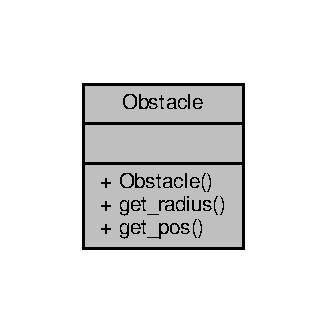
\includegraphics[width=157pt]{classObstacle__coll__graph}
\end{center}
\end{figure}
\subsection*{Public Member Functions}
\begin{DoxyCompactItemize}
\item 
\mbox{\Hypertarget{classObstacle_aa03143fb98cf3fe4f4fb67d1b450b33f}\label{classObstacle_aa03143fb98cf3fe4f4fb67d1b450b33f}} 
int {\bfseries get\+\_\+radius} ()
\item 
\mbox{\Hypertarget{classObstacle_a5589725dc457a030f92e73eb632ae205}\label{classObstacle_a5589725dc457a030f92e73eb632ae205}} 
std\+::pair$<$ double, double $>$ {\bfseries get\+\_\+pos} ()
\end{DoxyCompactItemize}


The documentation for this class was generated from the following file\+:\begin{DoxyCompactItemize}
\item 
/home/almqu071/\+C\+S\+C\+I3081/3081\+\_\+\+S19/repo-\/almqu071/labs/lab07\+\_\+style\+\_\+doxy/src/mainpage.\+h\end{DoxyCompactItemize}

\hypertarget{classrobot__land}{}\section{robot\+\_\+land Class Reference}
\label{classrobot__land}\index{robot\+\_\+land@{robot\+\_\+land}}


The main class for the simulation of a 2D world with many robots running around.  




{\ttfamily \#include $<$robot\+\_\+land.\+h$>$}



Collaboration diagram for robot\+\_\+land\+:\nopagebreak
\begin{figure}[H]
\begin{center}
\leavevmode
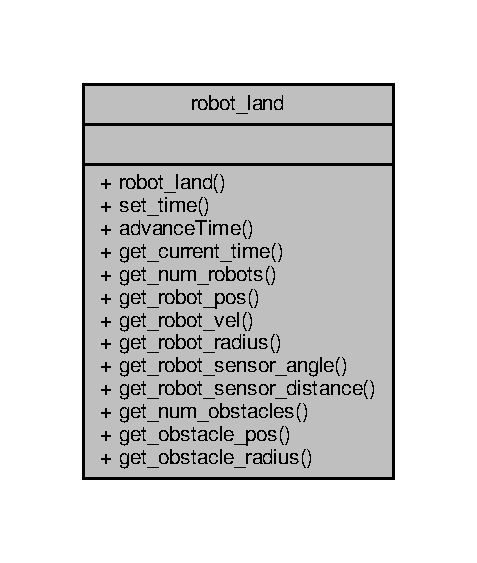
\includegraphics[width=229pt]{classrobot__land__coll__graph}
\end{center}
\end{figure}
\subsection*{Public Member Functions}
\begin{DoxyCompactItemize}
\item 
void \hyperlink{classrobot__land_a9b759efccbcae2be07ead240caec14cf}{set\+\_\+time} (double t)
\begin{DoxyCompactList}\small\item\em Set the simulation time for Robot\+Land. \end{DoxyCompactList}\item 
void \hyperlink{classrobot__land_af48446e7dafcf509fd3c13e66e17466b}{advance\+Time} (double dt)
\begin{DoxyCompactList}\small\item\em Advance the simulation by the specified \# of steps. \end{DoxyCompactList}\item 
\mbox{\Hypertarget{classrobot__land_a9469257602322310502bfe0298bea0e4}\label{classrobot__land_a9469257602322310502bfe0298bea0e4}} 
double \hyperlink{classrobot__land_a9469257602322310502bfe0298bea0e4}{get\+\_\+current\+\_\+time} (void)
\begin{DoxyCompactList}\small\item\em Get the current simulation time. \end{DoxyCompactList}\item 
\mbox{\Hypertarget{classrobot__land_a604710cec501348f61c009ed9066232e}\label{classrobot__land_a604710cec501348f61c009ed9066232e}} 
int {\bfseries get\+\_\+num\+\_\+robots} (void)
\item 
bool \hyperlink{classrobot__land_a600cee26e615092e6425e5f1f8544d8b}{get\+\_\+robot\+\_\+pos} (int id, double $\ast$x\+\_\+pos, double $\ast$y\+\_\+pos)
\begin{DoxyCompactList}\small\item\em Get the current position of the specified robot. Currently a stub. \end{DoxyCompactList}\item 
bool \hyperlink{classrobot__land_a2c12e8cb4cea6ca18db18b30b205b6a8}{get\+\_\+robot\+\_\+vel} (int id, double $\ast$x\+\_\+vel, double $\ast$y\+\_\+vel)
\begin{DoxyCompactList}\small\item\em Get the current velocity of the specified robot. Currently a stub. \end{DoxyCompactList}\item 
double \hyperlink{classrobot__land_a874897fdbb0d4bf54cd70226d3515bdd}{get\+\_\+robot\+\_\+radius} ()
\begin{DoxyCompactList}\small\item\em Get the radius of the specified robot. Currently a stub. \end{DoxyCompactList}\item 
double \hyperlink{classrobot__land_a9f874d4ea9cb32801af60413753a39f7}{get\+\_\+robot\+\_\+sensor\+\_\+angle} ()
\begin{DoxyCompactList}\small\item\em Get the angle of the specified robots sensor, in radians. Currently a stub. \end{DoxyCompactList}\item 
double \hyperlink{classrobot__land_a4bef892a1b2c7c6a539dfed5fd2abae5}{get\+\_\+robot\+\_\+sensor\+\_\+distance} ()
\begin{DoxyCompactList}\small\item\em Get the distance of a specified robot\textquotesingle{}s sensor. Currently a stub. \end{DoxyCompactList}\item 
int \hyperlink{classrobot__land_ab6edf762a971b54341c1d0740c2c431d}{get\+\_\+num\+\_\+obstacles} (void)
\begin{DoxyCompactList}\small\item\em Get the \# of obstacles currently in Robot\+Land. Currently a stub. \end{DoxyCompactList}\item 
bool \hyperlink{classrobot__land_ab9f49e83909a16ecc0aeae8f6fa6f673}{get\+\_\+obstacle\+\_\+pos} (int id, double $\ast$x\+\_\+pos, double $\ast$y\+\_\+pos)
\begin{DoxyCompactList}\small\item\em Get the position of the specified obstacle. Currently a stub. \end{DoxyCompactList}\item 
double \hyperlink{classrobot__land_aefbde3fcc92d17c9a048f496f2cd7454}{get\+\_\+obstacle\+\_\+radius} ()
\begin{DoxyCompactList}\small\item\em Get the radius of the specified obstacle. \end{DoxyCompactList}\end{DoxyCompactItemize}


\subsection{Detailed Description}
The main class for the simulation of a 2D world with many robots running around. 

\hyperlink{classRobotViewer}{Robot\+Viewer} or Tests call \hyperlink{classrobot__land_a9b759efccbcae2be07ead240caec14cf}{set\+\_\+time} and advance\+\_\+time to control the simulation and use the get$\ast$() functions to read out the current state of the simulation (i.\+e., the current positions and orientations of robots and obstacles).

For now, Robot\+Land is hard coded to run a simulation of two robots running around in a circle. You can see their sensors, but they don\textquotesingle{}t yet respond to each other or to obstacles. 

\subsection{Member Function Documentation}
\mbox{\Hypertarget{classrobot__land_af48446e7dafcf509fd3c13e66e17466b}\label{classrobot__land_af48446e7dafcf509fd3c13e66e17466b}} 
\index{robot\+\_\+land@{robot\+\_\+land}!advance\+Time@{advance\+Time}}
\index{advance\+Time@{advance\+Time}!robot\+\_\+land@{robot\+\_\+land}}
\subsubsection{\texorpdfstring{advance\+Time()}{advanceTime()}}
{\footnotesize\ttfamily void robot\+\_\+land\+::advance\+Time (\begin{DoxyParamCaption}\item[{double}]{dt }\end{DoxyParamCaption})\hspace{0.3cm}{\ttfamily [inline]}}



Advance the simulation by the specified \# of steps. 


\begin{DoxyParams}[1]{Parameters}
\mbox{\tt in}  & {\em dt} & The \# of steps to increment by. \\
\hline
\end{DoxyParams}
\mbox{\Hypertarget{classrobot__land_ab6edf762a971b54341c1d0740c2c431d}\label{classrobot__land_ab6edf762a971b54341c1d0740c2c431d}} 
\index{robot\+\_\+land@{robot\+\_\+land}!get\+\_\+num\+\_\+obstacles@{get\+\_\+num\+\_\+obstacles}}
\index{get\+\_\+num\+\_\+obstacles@{get\+\_\+num\+\_\+obstacles}!robot\+\_\+land@{robot\+\_\+land}}
\subsubsection{\texorpdfstring{get\+\_\+num\+\_\+obstacles()}{get\_num\_obstacles()}}
{\footnotesize\ttfamily int robot\+\_\+land\+::get\+\_\+num\+\_\+obstacles (\begin{DoxyParamCaption}\item[{void}]{ }\end{DoxyParamCaption})}



Get the \# of obstacles currently in Robot\+Land. Currently a stub. 

\begin{DoxyRefDesc}{Todo}
\item[\hyperlink{todo__todo000008}{Todo}]\+: Actually implement this.\end{DoxyRefDesc}


\begin{DoxyReturn}{Returns}
The \# of obstacles. 
\end{DoxyReturn}
\mbox{\Hypertarget{classrobot__land_ab9f49e83909a16ecc0aeae8f6fa6f673}\label{classrobot__land_ab9f49e83909a16ecc0aeae8f6fa6f673}} 
\index{robot\+\_\+land@{robot\+\_\+land}!get\+\_\+obstacle\+\_\+pos@{get\+\_\+obstacle\+\_\+pos}}
\index{get\+\_\+obstacle\+\_\+pos@{get\+\_\+obstacle\+\_\+pos}!robot\+\_\+land@{robot\+\_\+land}}
\subsubsection{\texorpdfstring{get\+\_\+obstacle\+\_\+pos()}{get\_obstacle\_pos()}}
{\footnotesize\ttfamily bool robot\+\_\+land\+::get\+\_\+obstacle\+\_\+pos (\begin{DoxyParamCaption}\item[{int}]{id,  }\item[{double $\ast$}]{x\+\_\+pos,  }\item[{double $\ast$}]{y\+\_\+pos }\end{DoxyParamCaption})}



Get the position of the specified obstacle. Currently a stub. 

\begin{DoxyRefDesc}{Todo}
\item[\hyperlink{todo__todo000009}{Todo}]\+: Actually implement this.\end{DoxyRefDesc}



\begin{DoxyParams}[1]{Parameters}
\mbox{\tt in}  & {\em id} & The ID of the obstacle. \\
\hline
\mbox{\tt out}  & {\em x\+\_\+pos} & The X component of the position. \\
\hline
\mbox{\tt out}  & {\em y\+\_\+pos} & The Y component of the position.\\
\hline
\end{DoxyParams}
\begin{DoxyReturn}{Returns}

\end{DoxyReturn}
\begin{DoxyRefDesc}{Todo}
\item[\hyperlink{todo__todo000010}{Todo}]What does this mean? \end{DoxyRefDesc}
\mbox{\Hypertarget{classrobot__land_aefbde3fcc92d17c9a048f496f2cd7454}\label{classrobot__land_aefbde3fcc92d17c9a048f496f2cd7454}} 
\index{robot\+\_\+land@{robot\+\_\+land}!get\+\_\+obstacle\+\_\+radius@{get\+\_\+obstacle\+\_\+radius}}
\index{get\+\_\+obstacle\+\_\+radius@{get\+\_\+obstacle\+\_\+radius}!robot\+\_\+land@{robot\+\_\+land}}
\subsubsection{\texorpdfstring{get\+\_\+obstacle\+\_\+radius()}{get\_obstacle\_radius()}}
{\footnotesize\ttfamily double robot\+\_\+land\+::get\+\_\+obstacle\+\_\+radius (\begin{DoxyParamCaption}{ }\end{DoxyParamCaption})}



Get the radius of the specified obstacle. 


\begin{DoxyParams}[1]{Parameters}
\mbox{\tt in}  & {\em id} & The ID of the obstacle.\\
\hline
\end{DoxyParams}
\begin{DoxyReturn}{Returns}
The obstacle\textquotesingle{}s radius. 
\end{DoxyReturn}
\mbox{\Hypertarget{classrobot__land_a600cee26e615092e6425e5f1f8544d8b}\label{classrobot__land_a600cee26e615092e6425e5f1f8544d8b}} 
\index{robot\+\_\+land@{robot\+\_\+land}!get\+\_\+robot\+\_\+pos@{get\+\_\+robot\+\_\+pos}}
\index{get\+\_\+robot\+\_\+pos@{get\+\_\+robot\+\_\+pos}!robot\+\_\+land@{robot\+\_\+land}}
\subsubsection{\texorpdfstring{get\+\_\+robot\+\_\+pos()}{get\_robot\_pos()}}
{\footnotesize\ttfamily bool robot\+\_\+land\+::get\+\_\+robot\+\_\+pos (\begin{DoxyParamCaption}\item[{int}]{id,  }\item[{double $\ast$}]{x\+\_\+pos,  }\item[{double $\ast$}]{y\+\_\+pos }\end{DoxyParamCaption})}



Get the current position of the specified robot. Currently a stub. 

\begin{DoxyRefDesc}{Todo}
\item[\hyperlink{todo__todo000001}{Todo}]\+: Actually implement this.\end{DoxyRefDesc}



\begin{DoxyParams}[1]{Parameters}
\mbox{\tt in}  & {\em id} & The ID of the robot. \\
\hline
\mbox{\tt out}  & {\em x\+\_\+pos} & The X position of the robot. \\
\hline
\mbox{\tt out}  & {\em y\+\_\+pos} & The Y position of the robot.\\
\hline
\end{DoxyParams}
\begin{DoxyReturn}{Returns}

\end{DoxyReturn}
\begin{DoxyRefDesc}{Todo}
\item[\hyperlink{todo__todo000002}{Todo}]\+: What does this mean? \end{DoxyRefDesc}
\mbox{\Hypertarget{classrobot__land_a874897fdbb0d4bf54cd70226d3515bdd}\label{classrobot__land_a874897fdbb0d4bf54cd70226d3515bdd}} 
\index{robot\+\_\+land@{robot\+\_\+land}!get\+\_\+robot\+\_\+radius@{get\+\_\+robot\+\_\+radius}}
\index{get\+\_\+robot\+\_\+radius@{get\+\_\+robot\+\_\+radius}!robot\+\_\+land@{robot\+\_\+land}}
\subsubsection{\texorpdfstring{get\+\_\+robot\+\_\+radius()}{get\_robot\_radius()}}
{\footnotesize\ttfamily double robot\+\_\+land\+::get\+\_\+robot\+\_\+radius (\begin{DoxyParamCaption}{ }\end{DoxyParamCaption})}



Get the radius of the specified robot. Currently a stub. 

\begin{DoxyRefDesc}{Todo}
\item[\hyperlink{todo__todo000005}{Todo}]\+: Actually implement this.\end{DoxyRefDesc}



\begin{DoxyParams}[1]{Parameters}
\mbox{\tt in}  & {\em id} & The ID of the robot.\\
\hline
\end{DoxyParams}
\begin{DoxyReturn}{Returns}
The robot\textquotesingle{}s radius. 
\end{DoxyReturn}
\mbox{\Hypertarget{classrobot__land_a9f874d4ea9cb32801af60413753a39f7}\label{classrobot__land_a9f874d4ea9cb32801af60413753a39f7}} 
\index{robot\+\_\+land@{robot\+\_\+land}!get\+\_\+robot\+\_\+sensor\+\_\+angle@{get\+\_\+robot\+\_\+sensor\+\_\+angle}}
\index{get\+\_\+robot\+\_\+sensor\+\_\+angle@{get\+\_\+robot\+\_\+sensor\+\_\+angle}!robot\+\_\+land@{robot\+\_\+land}}
\subsubsection{\texorpdfstring{get\+\_\+robot\+\_\+sensor\+\_\+angle()}{get\_robot\_sensor\_angle()}}
{\footnotesize\ttfamily double robot\+\_\+land\+::get\+\_\+robot\+\_\+sensor\+\_\+angle (\begin{DoxyParamCaption}{ }\end{DoxyParamCaption})}



Get the angle of the specified robots sensor, in radians. Currently a stub. 

\begin{DoxyRefDesc}{Todo}
\item[\hyperlink{todo__todo000006}{Todo}]\+: Actually implement this.\end{DoxyRefDesc}


\begin{DoxyReturn}{Returns}
The sensor angle in radians, 
\end{DoxyReturn}
\mbox{\Hypertarget{classrobot__land_a4bef892a1b2c7c6a539dfed5fd2abae5}\label{classrobot__land_a4bef892a1b2c7c6a539dfed5fd2abae5}} 
\index{robot\+\_\+land@{robot\+\_\+land}!get\+\_\+robot\+\_\+sensor\+\_\+distance@{get\+\_\+robot\+\_\+sensor\+\_\+distance}}
\index{get\+\_\+robot\+\_\+sensor\+\_\+distance@{get\+\_\+robot\+\_\+sensor\+\_\+distance}!robot\+\_\+land@{robot\+\_\+land}}
\subsubsection{\texorpdfstring{get\+\_\+robot\+\_\+sensor\+\_\+distance()}{get\_robot\_sensor\_distance()}}
{\footnotesize\ttfamily double robot\+\_\+land\+::get\+\_\+robot\+\_\+sensor\+\_\+distance (\begin{DoxyParamCaption}{ }\end{DoxyParamCaption})}



Get the distance of a specified robot\textquotesingle{}s sensor. Currently a stub. 

\begin{DoxyRefDesc}{Todo}
\item[\hyperlink{todo__todo000007}{Todo}]\+: Actually implement this.\end{DoxyRefDesc}


\begin{DoxyReturn}{Returns}
The sensor distance. 
\end{DoxyReturn}
\mbox{\Hypertarget{classrobot__land_a2c12e8cb4cea6ca18db18b30b205b6a8}\label{classrobot__land_a2c12e8cb4cea6ca18db18b30b205b6a8}} 
\index{robot\+\_\+land@{robot\+\_\+land}!get\+\_\+robot\+\_\+vel@{get\+\_\+robot\+\_\+vel}}
\index{get\+\_\+robot\+\_\+vel@{get\+\_\+robot\+\_\+vel}!robot\+\_\+land@{robot\+\_\+land}}
\subsubsection{\texorpdfstring{get\+\_\+robot\+\_\+vel()}{get\_robot\_vel()}}
{\footnotesize\ttfamily bool robot\+\_\+land\+::get\+\_\+robot\+\_\+vel (\begin{DoxyParamCaption}\item[{int}]{id,  }\item[{double $\ast$}]{x\+\_\+vel,  }\item[{double $\ast$}]{y\+\_\+vel }\end{DoxyParamCaption})}



Get the current velocity of the specified robot. Currently a stub. 

\begin{DoxyRefDesc}{Todo}
\item[\hyperlink{todo__todo000003}{Todo}]Actually implement this.\end{DoxyRefDesc}



\begin{DoxyParams}[1]{Parameters}
\mbox{\tt in}  & {\em id} & The ID of the robot. \\
\hline
\mbox{\tt out}  & {\em x\+\_\+vel} & The X component of velocity. \\
\hline
\mbox{\tt out}  & {\em y\+\_\+vel} & The Y component of velocity.\\
\hline
\end{DoxyParams}
\begin{DoxyReturn}{Returns}

\end{DoxyReturn}
\begin{DoxyRefDesc}{Todo}
\item[\hyperlink{todo__todo000004}{Todo}]what does this mean? \end{DoxyRefDesc}
\mbox{\Hypertarget{classrobot__land_a9b759efccbcae2be07ead240caec14cf}\label{classrobot__land_a9b759efccbcae2be07ead240caec14cf}} 
\index{robot\+\_\+land@{robot\+\_\+land}!set\+\_\+time@{set\+\_\+time}}
\index{set\+\_\+time@{set\+\_\+time}!robot\+\_\+land@{robot\+\_\+land}}
\subsubsection{\texorpdfstring{set\+\_\+time()}{set\_time()}}
{\footnotesize\ttfamily void robot\+\_\+land\+::set\+\_\+time (\begin{DoxyParamCaption}\item[{double}]{t }\end{DoxyParamCaption})\hspace{0.3cm}{\ttfamily [inline]}}



Set the simulation time for Robot\+Land. 

This function will be used mainly for testing purposes, as time flows in a steady forward direction in general simulation.


\begin{DoxyParams}[1]{Parameters}
\mbox{\tt in}  & {\em t} & The new simulation time. \\
\hline
\end{DoxyParams}


The documentation for this class was generated from the following files\+:\begin{DoxyCompactItemize}
\item 
/home/almqu071/\+C\+S\+C\+I3081/3081\+\_\+\+S19/repo-\/almqu071/labs/lab07\+\_\+style\+\_\+doxy/src/\hyperlink{robot__land_8h}{robot\+\_\+land.\+h}\item 
/home/almqu071/\+C\+S\+C\+I3081/3081\+\_\+\+S19/repo-\/almqu071/labs/lab07\+\_\+style\+\_\+doxy/src/\hyperlink{robot__land_8cc}{robot\+\_\+land.\+cc}\end{DoxyCompactItemize}

\hypertarget{classRobotViewer}{}\section{Robot\+Viewer Class Reference}
\label{classRobotViewer}\index{Robot\+Viewer@{Robot\+Viewer}}


An application that uses the cs3081 Simple\+Graphics library to open up a window that includes a few buttons for controlling the simulation and can be used to draw circles and other computer graphics.  




{\ttfamily \#include $<$robot\+\_\+viewer.\+h$>$}



Inheritance diagram for Robot\+Viewer\+:\nopagebreak
\begin{figure}[H]
\begin{center}
\leavevmode
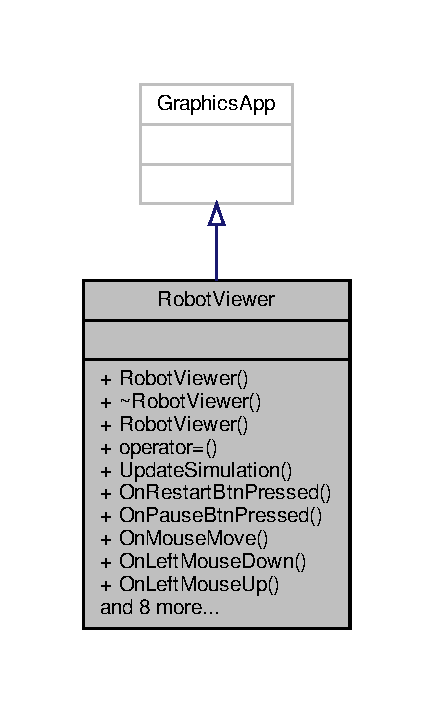
\includegraphics[width=208pt]{classRobotViewer__inherit__graph}
\end{center}
\end{figure}


Collaboration diagram for Robot\+Viewer\+:\nopagebreak
\begin{figure}[H]
\begin{center}
\leavevmode
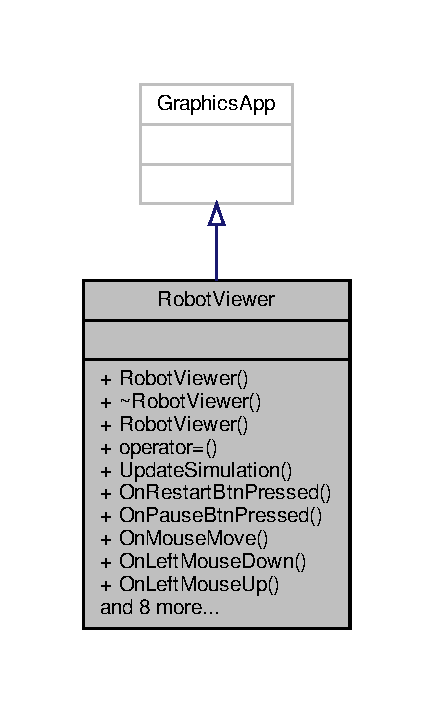
\includegraphics[width=208pt]{classRobotViewer__coll__graph}
\end{center}
\end{figure}
\subsection*{Public Member Functions}
\begin{DoxyCompactItemize}
\item 
\mbox{\Hypertarget{classRobotViewer_a722235e9d5cc60161e15dd189bf79566}\label{classRobotViewer_a722235e9d5cc60161e15dd189bf79566}} 
{\bfseries Robot\+Viewer} (const \hyperlink{classRobotViewer}{Robot\+Viewer} \&other)=delete
\item 
\mbox{\Hypertarget{classRobotViewer_a4e7109141d452ea091e776d0069e03fb}\label{classRobotViewer_a4e7109141d452ea091e776d0069e03fb}} 
\hyperlink{classRobotViewer}{Robot\+Viewer} \& {\bfseries operator=} (const \hyperlink{classRobotViewer}{Robot\+Viewer} \&other)=delete
\item 
\mbox{\Hypertarget{classRobotViewer_a05c15913e55cd6925a089ce7c1fa5a55}\label{classRobotViewer_a05c15913e55cd6925a089ce7c1fa5a55}} 
void {\bfseries Update\+Simulation} (double dt) override
\item 
\mbox{\Hypertarget{classRobotViewer_a53b22985d65f9d2feb02deef32346030}\label{classRobotViewer_a53b22985d65f9d2feb02deef32346030}} 
void \hyperlink{classRobotViewer_a53b22985d65f9d2feb02deef32346030}{On\+Restart\+Btn\+Pressed} ()
\begin{DoxyCompactList}\small\item\em Handle the user pressing the restart button on the G\+UI. \end{DoxyCompactList}\item 
\mbox{\Hypertarget{classRobotViewer_ac1797fc2a436b9e176baf526ca9e9936}\label{classRobotViewer_ac1797fc2a436b9e176baf526ca9e9936}} 
void \hyperlink{classRobotViewer_ac1797fc2a436b9e176baf526ca9e9936}{On\+Pause\+Btn\+Pressed} ()
\begin{DoxyCompactList}\small\item\em Handle the user pressing the pause button on the G\+UI. \end{DoxyCompactList}\item 
void \hyperlink{classRobotViewer_ae3b11d89a8f596d43bd7127ed7cfccf5}{On\+Mouse\+Move} (\+\_\+\+\_\+unused const Point2 \&pos, \+\_\+\+\_\+unused const Vector2 \&delta) override
\begin{DoxyCompactList}\small\item\em Called each time the mouse moves on the screen within the G\+UI window. \end{DoxyCompactList}\item 
void \hyperlink{classRobotViewer_a51776dc0f3c06be3e459e2669a7bd3ff}{On\+Left\+Mouse\+Down} (\+\_\+\+\_\+unused const Point2 \&pos) override
\begin{DoxyCompactList}\small\item\em Called each time the left mouse button is clicked. \end{DoxyCompactList}\item 
void \hyperlink{classRobotViewer_a4b9372334e89152c2f8daf2cc2687943}{On\+Left\+Mouse\+Up} (\+\_\+\+\_\+unused const Point2 \&pos) override
\begin{DoxyCompactList}\small\item\em Called each time the left mouse button is released. \end{DoxyCompactList}\item 
void \hyperlink{classRobotViewer_ab5420b89be50106eefcbc44dece71e74}{On\+Right\+Mouse\+Down} (\+\_\+\+\_\+unused const Point2 \&pos) override
\begin{DoxyCompactList}\small\item\em Called each time the right mouse button is clicked. \end{DoxyCompactList}\item 
void \hyperlink{classRobotViewer_afe613a2bd8c13810327cf5344dac1a5e}{On\+Right\+Mouse\+Up} (\+\_\+\+\_\+unused const Point2 \&pos) override
\begin{DoxyCompactList}\small\item\em Called each time the right mouse button is released. \end{DoxyCompactList}\item 
void \hyperlink{classRobotViewer_a5a5e4be05ae7a8b3d137a3388638ad63}{On\+Key\+Down} (\+\_\+\+\_\+unused const char $\ast$c, \+\_\+\+\_\+unused int modifiers) override
\begin{DoxyCompactList}\small\item\em Called each time a character key is pressed. \end{DoxyCompactList}\item 
void \hyperlink{classRobotViewer_a7607dc80b550f1e1f2d88cccb21fe6af}{On\+Key\+Up} (\+\_\+\+\_\+unused const char $\ast$c, \+\_\+\+\_\+unused int modifiers) override
\begin{DoxyCompactList}\small\item\em Called each time a character key is released. \end{DoxyCompactList}\item 
void \hyperlink{classRobotViewer_a76911b260748dc4b4d5187fd85e23b71}{On\+Special\+Key\+Down} (\+\_\+\+\_\+unused int key, \+\_\+\+\_\+unused int scancode, \+\_\+\+\_\+unused int modifiers) override
\begin{DoxyCompactList}\small\item\em Called each time a special (non-\/alphabetic) key is pressed. \end{DoxyCompactList}\item 
void \hyperlink{classRobotViewer_a4d81343908c8e2ef4e48c6320b52ffdd}{On\+Special\+Key\+Up} (\+\_\+\+\_\+unused int key, \+\_\+\+\_\+unused int scancode, \+\_\+\+\_\+unused int modifiers) override
\begin{DoxyCompactList}\small\item\em Called each time a special (non-\/alphabetic) key is released. \end{DoxyCompactList}\item 
void \hyperlink{classRobotViewer_ac67e2c6bc6f4ddc6c50d4c7e05d99662}{Draw\+Using\+Nano\+VG} (N\+V\+Gcontext $\ast$ctx) override
\begin{DoxyCompactList}\small\item\em Draw the arena with all robots, obstacles using nanogui. \end{DoxyCompactList}\item 
\mbox{\Hypertarget{classRobotViewer_accb905122b66ed5a084c77b078216083}\label{classRobotViewer_accb905122b66ed5a084c77b078216083}} 
void \hyperlink{classRobotViewer_accb905122b66ed5a084c77b078216083}{Draw\+Using\+Open\+GL} (void) override
\begin{DoxyCompactList}\small\item\em Draw using Open\+GL. This callback had to be defined, but we are doing all drawing with nanovg in this application, so it is empty. \end{DoxyCompactList}\end{DoxyCompactItemize}


\subsection{Detailed Description}
An application that uses the cs3081 Simple\+Graphics library to open up a window that includes a few buttons for controlling the simulation and can be used to draw circles and other computer graphics. 

After constructing a new \hyperlink{classRobotViewer}{Robot\+Viewer}, call Run() to start and run the application. Run() will not return until the application window is closed. Make sure that you call cs3081\+::\+Init\+Graphics() before creating the \hyperlink{classRobotViewer}{Robot\+Viewer} app. Example\+:


\begin{DoxyCode}
\textcolor{keywordtype}{int} main(\textcolor{keywordtype}{int} argc, \textcolor{keywordtype}{char} **argv) \{
    cs3081::InitGraphics();
    \hyperlink{classRobotViewer}{RobotViewer} *app = \textcolor{keyword}{new} \hyperlink{classRobotViewer}{RobotViewer}();
    app->Run();
    cs3081::ShutdownGraphics();
    \textcolor{keywordflow}{return} 0;
\}
\end{DoxyCode}


While the window is open Update\+Simulation() will be called repeatedly, once per frame. Fill this in to update your simulation or perform any other processing that should happen over time as the simulation progresses.

Fill in the On$\ast$() methods as desired to respond to user input events.

Fill in the Draw$\ast$() methods to draw graphics to the screen using either the nanovg library or raw Open\+GL. 

\subsection{Member Function Documentation}
\mbox{\Hypertarget{classRobotViewer_ac67e2c6bc6f4ddc6c50d4c7e05d99662}\label{classRobotViewer_ac67e2c6bc6f4ddc6c50d4c7e05d99662}} 
\index{Robot\+Viewer@{Robot\+Viewer}!Draw\+Using\+Nano\+VG@{Draw\+Using\+Nano\+VG}}
\index{Draw\+Using\+Nano\+VG@{Draw\+Using\+Nano\+VG}!Robot\+Viewer@{Robot\+Viewer}}
\subsubsection{\texorpdfstring{Draw\+Using\+Nano\+V\+G()}{DrawUsingNanoVG()}}
{\footnotesize\ttfamily void Robot\+Viewer\+::\+Draw\+Using\+Nano\+VG (\begin{DoxyParamCaption}\item[{N\+V\+Gcontext $\ast$}]{ctx }\end{DoxyParamCaption})\hspace{0.3cm}{\ttfamily [override]}}



Draw the arena with all robots, obstacles using nanogui. 


\begin{DoxyParams}[1]{Parameters}
\mbox{\tt in}  & {\em ctx} & Context for nanogui. \\
\hline
\end{DoxyParams}
\mbox{\Hypertarget{classRobotViewer_a5a5e4be05ae7a8b3d137a3388638ad63}\label{classRobotViewer_a5a5e4be05ae7a8b3d137a3388638ad63}} 
\index{Robot\+Viewer@{Robot\+Viewer}!On\+Key\+Down@{On\+Key\+Down}}
\index{On\+Key\+Down@{On\+Key\+Down}!Robot\+Viewer@{Robot\+Viewer}}
\subsubsection{\texorpdfstring{On\+Key\+Down()}{OnKeyDown()}}
{\footnotesize\ttfamily void Robot\+Viewer\+::\+On\+Key\+Down (\begin{DoxyParamCaption}\item[{\+\_\+\+\_\+unused const char $\ast$}]{c,  }\item[{\+\_\+\+\_\+unused int}]{modifiers }\end{DoxyParamCaption})\hspace{0.3cm}{\ttfamily [inline]}, {\ttfamily [override]}}



Called each time a character key is pressed. 

This function is a stub.


\begin{DoxyParams}[1]{Parameters}
\mbox{\tt in}  & {\em c} & Character representing a key that was pressed. \\
\hline
\mbox{\tt in}  & {\em modifiers} & Any modifier keys that were also pressed. \\
\hline
\end{DoxyParams}
\mbox{\Hypertarget{classRobotViewer_a7607dc80b550f1e1f2d88cccb21fe6af}\label{classRobotViewer_a7607dc80b550f1e1f2d88cccb21fe6af}} 
\index{Robot\+Viewer@{Robot\+Viewer}!On\+Key\+Up@{On\+Key\+Up}}
\index{On\+Key\+Up@{On\+Key\+Up}!Robot\+Viewer@{Robot\+Viewer}}
\subsubsection{\texorpdfstring{On\+Key\+Up()}{OnKeyUp()}}
{\footnotesize\ttfamily void Robot\+Viewer\+::\+On\+Key\+Up (\begin{DoxyParamCaption}\item[{\+\_\+\+\_\+unused const char $\ast$}]{c,  }\item[{\+\_\+\+\_\+unused int}]{modifiers }\end{DoxyParamCaption})\hspace{0.3cm}{\ttfamily [inline]}, {\ttfamily [override]}}



Called each time a character key is released. 

This function is a stub.


\begin{DoxyParams}[1]{Parameters}
\mbox{\tt in}  & {\em c} & Character representing a key that was released. \\
\hline
\mbox{\tt in}  & {\em modifiers} & Any modifier keys that were held with the key. \\
\hline
\end{DoxyParams}
\mbox{\Hypertarget{classRobotViewer_a51776dc0f3c06be3e459e2669a7bd3ff}\label{classRobotViewer_a51776dc0f3c06be3e459e2669a7bd3ff}} 
\index{Robot\+Viewer@{Robot\+Viewer}!On\+Left\+Mouse\+Down@{On\+Left\+Mouse\+Down}}
\index{On\+Left\+Mouse\+Down@{On\+Left\+Mouse\+Down}!Robot\+Viewer@{Robot\+Viewer}}
\subsubsection{\texorpdfstring{On\+Left\+Mouse\+Down()}{OnLeftMouseDown()}}
{\footnotesize\ttfamily void Robot\+Viewer\+::\+On\+Left\+Mouse\+Down (\begin{DoxyParamCaption}\item[{\+\_\+\+\_\+unused const Point2 \&}]{pos }\end{DoxyParamCaption})\hspace{0.3cm}{\ttfamily [inline]}, {\ttfamily [override]}}



Called each time the left mouse button is clicked. 

Origin is at the lower left of the window. This function is a stub.


\begin{DoxyParams}[1]{Parameters}
\mbox{\tt in}  & {\em pos} & The position of the release. \\
\hline
\end{DoxyParams}
\mbox{\Hypertarget{classRobotViewer_a4b9372334e89152c2f8daf2cc2687943}\label{classRobotViewer_a4b9372334e89152c2f8daf2cc2687943}} 
\index{Robot\+Viewer@{Robot\+Viewer}!On\+Left\+Mouse\+Up@{On\+Left\+Mouse\+Up}}
\index{On\+Left\+Mouse\+Up@{On\+Left\+Mouse\+Up}!Robot\+Viewer@{Robot\+Viewer}}
\subsubsection{\texorpdfstring{On\+Left\+Mouse\+Up()}{OnLeftMouseUp()}}
{\footnotesize\ttfamily void Robot\+Viewer\+::\+On\+Left\+Mouse\+Up (\begin{DoxyParamCaption}\item[{\+\_\+\+\_\+unused const Point2 \&}]{pos }\end{DoxyParamCaption})\hspace{0.3cm}{\ttfamily [inline]}, {\ttfamily [override]}}



Called each time the left mouse button is released. 

Origin is at the lower left of the window. This function is a stub.


\begin{DoxyParams}[1]{Parameters}
\mbox{\tt in}  & {\em pos} & The position of the release. \\
\hline
\end{DoxyParams}
\mbox{\Hypertarget{classRobotViewer_ae3b11d89a8f596d43bd7127ed7cfccf5}\label{classRobotViewer_ae3b11d89a8f596d43bd7127ed7cfccf5}} 
\index{Robot\+Viewer@{Robot\+Viewer}!On\+Mouse\+Move@{On\+Mouse\+Move}}
\index{On\+Mouse\+Move@{On\+Mouse\+Move}!Robot\+Viewer@{Robot\+Viewer}}
\subsubsection{\texorpdfstring{On\+Mouse\+Move()}{OnMouseMove()}}
{\footnotesize\ttfamily void Robot\+Viewer\+::\+On\+Mouse\+Move (\begin{DoxyParamCaption}\item[{\+\_\+\+\_\+unused const Point2 \&}]{pos,  }\item[{\+\_\+\+\_\+unused const Vector2 \&}]{delta }\end{DoxyParamCaption})\hspace{0.3cm}{\ttfamily [inline]}, {\ttfamily [override]}}



Called each time the mouse moves on the screen within the G\+UI window. 

Origin is at the lower left of the window. This function is a stub.


\begin{DoxyParams}[1]{Parameters}
\mbox{\tt in}  & {\em pos} & The position of the release. \\
\hline
\mbox{\tt in}  & {\em delta} & How far the mouse has moved. \\
\hline
\end{DoxyParams}
\mbox{\Hypertarget{classRobotViewer_ab5420b89be50106eefcbc44dece71e74}\label{classRobotViewer_ab5420b89be50106eefcbc44dece71e74}} 
\index{Robot\+Viewer@{Robot\+Viewer}!On\+Right\+Mouse\+Down@{On\+Right\+Mouse\+Down}}
\index{On\+Right\+Mouse\+Down@{On\+Right\+Mouse\+Down}!Robot\+Viewer@{Robot\+Viewer}}
\subsubsection{\texorpdfstring{On\+Right\+Mouse\+Down()}{OnRightMouseDown()}}
{\footnotesize\ttfamily void Robot\+Viewer\+::\+On\+Right\+Mouse\+Down (\begin{DoxyParamCaption}\item[{\+\_\+\+\_\+unused const Point2 \&}]{pos }\end{DoxyParamCaption})\hspace{0.3cm}{\ttfamily [inline]}, {\ttfamily [override]}}



Called each time the right mouse button is clicked. 

Origin is at the lower left of the window. This function is a stub.


\begin{DoxyParams}[1]{Parameters}
\mbox{\tt in}  & {\em pos} & The position of the release. \\
\hline
\end{DoxyParams}
\mbox{\Hypertarget{classRobotViewer_afe613a2bd8c13810327cf5344dac1a5e}\label{classRobotViewer_afe613a2bd8c13810327cf5344dac1a5e}} 
\index{Robot\+Viewer@{Robot\+Viewer}!On\+Right\+Mouse\+Up@{On\+Right\+Mouse\+Up}}
\index{On\+Right\+Mouse\+Up@{On\+Right\+Mouse\+Up}!Robot\+Viewer@{Robot\+Viewer}}
\subsubsection{\texorpdfstring{On\+Right\+Mouse\+Up()}{OnRightMouseUp()}}
{\footnotesize\ttfamily void Robot\+Viewer\+::\+On\+Right\+Mouse\+Up (\begin{DoxyParamCaption}\item[{\+\_\+\+\_\+unused const Point2 \&}]{pos }\end{DoxyParamCaption})\hspace{0.3cm}{\ttfamily [inline]}, {\ttfamily [override]}}



Called each time the right mouse button is released. 

Origin is at the lower left of the window. This function is a stub.


\begin{DoxyParams}[1]{Parameters}
\mbox{\tt in}  & {\em pos} & The position of the release. \\
\hline
\end{DoxyParams}
\mbox{\Hypertarget{classRobotViewer_a76911b260748dc4b4d5187fd85e23b71}\label{classRobotViewer_a76911b260748dc4b4d5187fd85e23b71}} 
\index{Robot\+Viewer@{Robot\+Viewer}!On\+Special\+Key\+Down@{On\+Special\+Key\+Down}}
\index{On\+Special\+Key\+Down@{On\+Special\+Key\+Down}!Robot\+Viewer@{Robot\+Viewer}}
\subsubsection{\texorpdfstring{On\+Special\+Key\+Down()}{OnSpecialKeyDown()}}
{\footnotesize\ttfamily void Robot\+Viewer\+::\+On\+Special\+Key\+Down (\begin{DoxyParamCaption}\item[{\+\_\+\+\_\+unused int}]{key,  }\item[{\+\_\+\+\_\+unused int}]{scancode,  }\item[{\+\_\+\+\_\+unused int}]{modifiers }\end{DoxyParamCaption})\hspace{0.3cm}{\ttfamily [inline]}, {\ttfamily [override]}}



Called each time a special (non-\/alphabetic) key is pressed. 

This function is a stub.


\begin{DoxyParams}[1]{Parameters}
\mbox{\tt in}  & {\em key} & The key that was pressed. \\
\hline
\mbox{\tt in}  & {\em scancode} & The scancode corresponding to the key. \\
\hline
\mbox{\tt in}  & {\em modifiers} & Any modifier keys that were also pressed. \\
\hline
\end{DoxyParams}
\mbox{\Hypertarget{classRobotViewer_a4d81343908c8e2ef4e48c6320b52ffdd}\label{classRobotViewer_a4d81343908c8e2ef4e48c6320b52ffdd}} 
\index{Robot\+Viewer@{Robot\+Viewer}!On\+Special\+Key\+Up@{On\+Special\+Key\+Up}}
\index{On\+Special\+Key\+Up@{On\+Special\+Key\+Up}!Robot\+Viewer@{Robot\+Viewer}}
\subsubsection{\texorpdfstring{On\+Special\+Key\+Up()}{OnSpecialKeyUp()}}
{\footnotesize\ttfamily void Robot\+Viewer\+::\+On\+Special\+Key\+Up (\begin{DoxyParamCaption}\item[{\+\_\+\+\_\+unused int}]{key,  }\item[{\+\_\+\+\_\+unused int}]{scancode,  }\item[{\+\_\+\+\_\+unused int}]{modifiers }\end{DoxyParamCaption})\hspace{0.3cm}{\ttfamily [inline]}, {\ttfamily [override]}}



Called each time a special (non-\/alphabetic) key is released. 

This function is a stub.


\begin{DoxyParams}[1]{Parameters}
\mbox{\tt in}  & {\em key} & The key that was released. \\
\hline
\mbox{\tt in}  & {\em scancode} & The scancode corresponding to the key. \\
\hline
\mbox{\tt in}  & {\em modifiers} & Any modifier keys that were also pressed. \\
\hline
\end{DoxyParams}


The documentation for this class was generated from the following files\+:\begin{DoxyCompactItemize}
\item 
/home/almqu071/\+C\+S\+C\+I3081/3081\+\_\+\+S19/repo-\/almqu071/labs/lab07\+\_\+style\+\_\+doxy/src/\hyperlink{robot__viewer_8h}{robot\+\_\+viewer.\+h}\item 
/home/almqu071/\+C\+S\+C\+I3081/3081\+\_\+\+S19/repo-\/almqu071/labs/lab07\+\_\+style\+\_\+doxy/src/\hyperlink{robot__viewer_8cc}{robot\+\_\+viewer.\+cc}\end{DoxyCompactItemize}

\chapter{File Documentation}
\hypertarget{main_8cc}{}\section{/home/almqu071/\+C\+S\+C\+I3081/3081\+\_\+\+S19/repo-\/almqu071/labs/lab07\+\_\+style\+\_\+doxy/src/main.cc File Reference}
\label{main_8cc}\index{/home/almqu071/\+C\+S\+C\+I3081/3081\+\_\+\+S19/repo-\/almqu071/labs/lab07\+\_\+style\+\_\+doxy/src/main.\+cc@{/home/almqu071/\+C\+S\+C\+I3081/3081\+\_\+\+S19/repo-\/almqu071/labs/lab07\+\_\+style\+\_\+doxy/src/main.\+cc}}
{\ttfamily \#include \char`\"{}src/robot\+\_\+viewer.\+h\char`\"{}}\newline
Include dependency graph for main.\+cc\+:\nopagebreak
\begin{figure}[H]
\begin{center}
\leavevmode
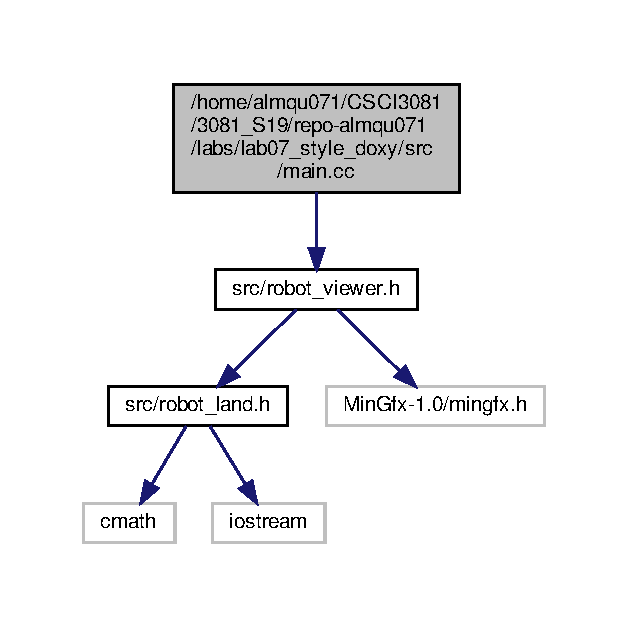
\includegraphics[width=302pt]{main_8cc__incl}
\end{center}
\end{figure}
\subsection*{Functions}
\begin{DoxyCompactItemize}
\item 
\mbox{\Hypertarget{main_8cc_a37539ad52260bcf576f148e7e141d4f2}\label{main_8cc_a37539ad52260bcf576f148e7e141d4f2}} 
int {\bfseries main} (\+\_\+\+\_\+unused int argc, \+\_\+\+\_\+unused char $\ast$$\ast$argv)
\end{DoxyCompactItemize}


\subsection{Detailed Description}
\begin{DoxyCopyright}{Copyright}
2018 3081 Staff, All rights reserved. 
\end{DoxyCopyright}

\hypertarget{robot__land_8cc}{}\section{/home/almqu071/\+C\+S\+C\+I3081/3081\+\_\+\+S19/repo-\/almqu071/labs/lab07\+\_\+style\+\_\+doxy/src/robot\+\_\+land.cc File Reference}
\label{robot__land_8cc}\index{/home/almqu071/\+C\+S\+C\+I3081/3081\+\_\+\+S19/repo-\/almqu071/labs/lab07\+\_\+style\+\_\+doxy/src/robot\+\_\+land.\+cc@{/home/almqu071/\+C\+S\+C\+I3081/3081\+\_\+\+S19/repo-\/almqu071/labs/lab07\+\_\+style\+\_\+doxy/src/robot\+\_\+land.\+cc}}
{\ttfamily \#include \char`\"{}src/robot\+\_\+land.\+h\char`\"{}}\newline
Include dependency graph for robot\+\_\+land.\+cc\+:\nopagebreak
\begin{figure}[H]
\begin{center}
\leavevmode
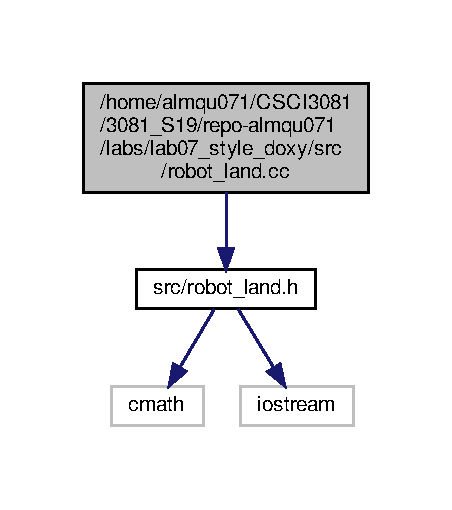
\includegraphics[width=217pt]{robot__land_8cc__incl}
\end{center}
\end{figure}


\subsection{Detailed Description}
\begin{DoxyCopyright}{Copyright}
201 3081 Staff, All rights reserved. 
\end{DoxyCopyright}

\hypertarget{robot__land_8h}{}\section{/home/almqu071/\+C\+S\+C\+I3081/3081\+\_\+\+S19/repo-\/almqu071/labs/lab07\+\_\+style\+\_\+doxy/src/robot\+\_\+land.h File Reference}
\label{robot__land_8h}\index{/home/almqu071/\+C\+S\+C\+I3081/3081\+\_\+\+S19/repo-\/almqu071/labs/lab07\+\_\+style\+\_\+doxy/src/robot\+\_\+land.\+h@{/home/almqu071/\+C\+S\+C\+I3081/3081\+\_\+\+S19/repo-\/almqu071/labs/lab07\+\_\+style\+\_\+doxy/src/robot\+\_\+land.\+h}}
{\ttfamily \#include $<$cmath$>$}\newline
{\ttfamily \#include $<$iostream$>$}\newline
Include dependency graph for robot\+\_\+land.\+h\+:\nopagebreak
\begin{figure}[H]
\begin{center}
\leavevmode
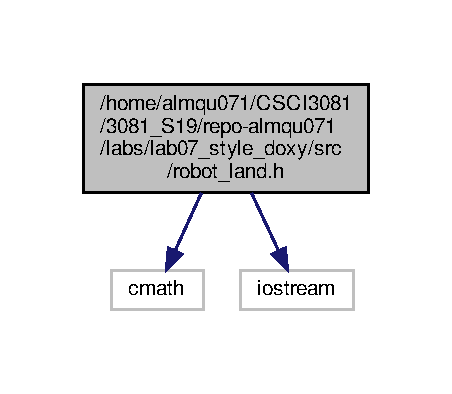
\includegraphics[width=217pt]{robot__land_8h__incl}
\end{center}
\end{figure}
This graph shows which files directly or indirectly include this file\+:\nopagebreak
\begin{figure}[H]
\begin{center}
\leavevmode
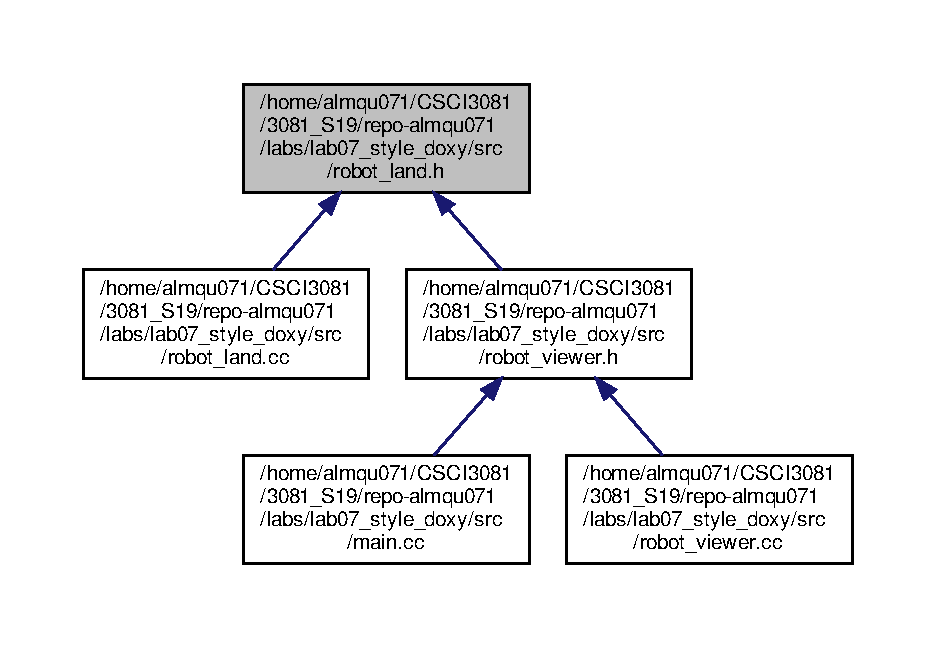
\includegraphics[width=350pt]{robot__land_8h__dep__incl}
\end{center}
\end{figure}
\subsection*{Classes}
\begin{DoxyCompactItemize}
\item 
class \hyperlink{classrobot__land}{robot\+\_\+land}
\begin{DoxyCompactList}\small\item\em The main class for the simulation of a 2D world with many robots running around. \end{DoxyCompactList}\end{DoxyCompactItemize}
\subsection*{Macros}
\begin{DoxyCompactItemize}
\item 
\mbox{\Hypertarget{robot__land_8h_a2e3484535ee610c8e19e9859563abe48}\label{robot__land_8h_a2e3484535ee610c8e19e9859563abe48}} 
\#define {\bfseries \+\_\+\+\_\+unused}~\+\_\+\+\_\+attribute\+\_\+\+\_\+((unused))
\end{DoxyCompactItemize}


\subsection{Detailed Description}
\begin{DoxyCopyright}{Copyright}
2017 3081 Staff, All rights reserved. 
\end{DoxyCopyright}

\hypertarget{robot__viewer_8cc}{}\section{/home/almqu071/\+C\+S\+C\+I3081/3081\+\_\+\+S19/repo-\/almqu071/labs/lab07\+\_\+style\+\_\+doxy/src/robot\+\_\+viewer.cc File Reference}
\label{robot__viewer_8cc}\index{/home/almqu071/\+C\+S\+C\+I3081/3081\+\_\+\+S19/repo-\/almqu071/labs/lab07\+\_\+style\+\_\+doxy/src/robot\+\_\+viewer.\+cc@{/home/almqu071/\+C\+S\+C\+I3081/3081\+\_\+\+S19/repo-\/almqu071/labs/lab07\+\_\+style\+\_\+doxy/src/robot\+\_\+viewer.\+cc}}
{\ttfamily \#include \char`\"{}src/robot\+\_\+viewer.\+h\char`\"{}}\newline
{\ttfamily \#include $<$iostream$>$}\newline
{\ttfamily \#include $<$string$>$}\newline
Include dependency graph for robot\+\_\+viewer.\+cc\+:\nopagebreak
\begin{figure}[H]
\begin{center}
\leavevmode
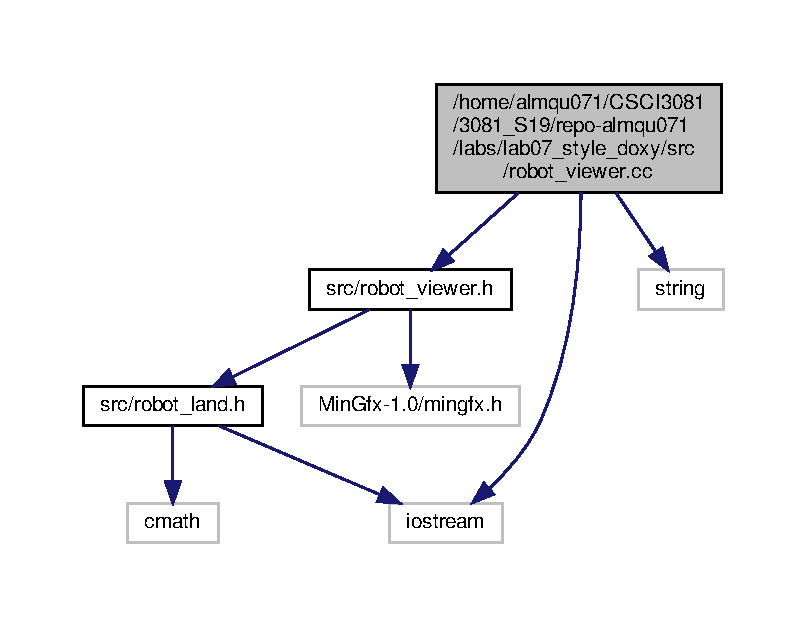
\includegraphics[width=350pt]{robot__viewer_8cc__incl}
\end{center}
\end{figure}


\subsection{Detailed Description}
\begin{DoxyCopyright}{Copyright}
2018 3081 Staff, All rights reserved. 
\end{DoxyCopyright}

\hypertarget{robot__viewer_8h}{}\section{/home/almqu071/\+C\+S\+C\+I3081/3081\+\_\+\+S19/repo-\/almqu071/labs/lab07\+\_\+style\+\_\+doxy/src/robot\+\_\+viewer.h File Reference}
\label{robot__viewer_8h}\index{/home/almqu071/\+C\+S\+C\+I3081/3081\+\_\+\+S19/repo-\/almqu071/labs/lab07\+\_\+style\+\_\+doxy/src/robot\+\_\+viewer.\+h@{/home/almqu071/\+C\+S\+C\+I3081/3081\+\_\+\+S19/repo-\/almqu071/labs/lab07\+\_\+style\+\_\+doxy/src/robot\+\_\+viewer.\+h}}
{\ttfamily \#include \char`\"{}src/robot\+\_\+land.\+h\char`\"{}}\newline
{\ttfamily \#include $<$Min\+Gfx-\/1.\+0/mingfx.\+h$>$}\newline
Include dependency graph for robot\+\_\+viewer.\+h\+:\nopagebreak
\begin{figure}[H]
\begin{center}
\leavevmode
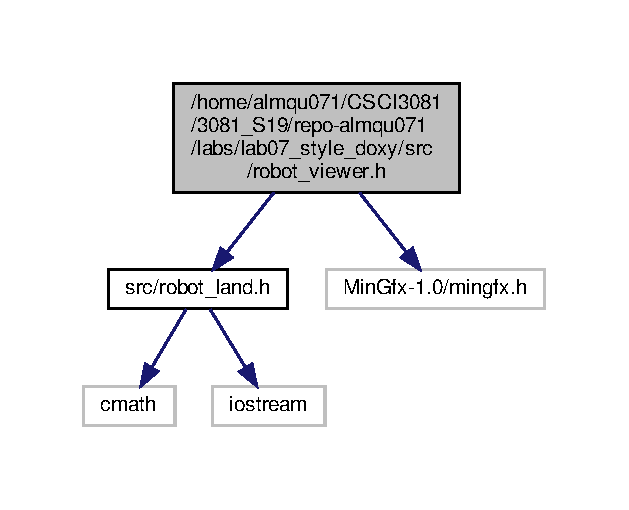
\includegraphics[width=302pt]{robot__viewer_8h__incl}
\end{center}
\end{figure}
This graph shows which files directly or indirectly include this file\+:\nopagebreak
\begin{figure}[H]
\begin{center}
\leavevmode
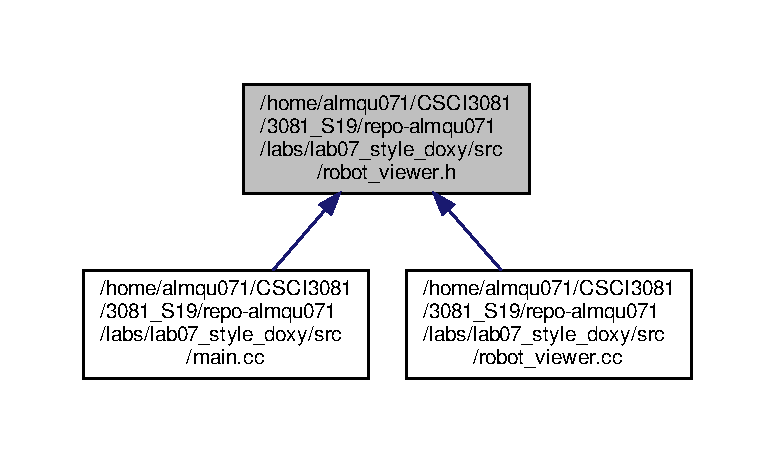
\includegraphics[width=350pt]{robot__viewer_8h__dep__incl}
\end{center}
\end{figure}
\subsection*{Classes}
\begin{DoxyCompactItemize}
\item 
class \hyperlink{classRobotViewer}{Robot\+Viewer}
\begin{DoxyCompactList}\small\item\em An application that uses the cs3081 Simple\+Graphics library to open up a window that includes a few buttons for controlling the simulation and can be used to draw circles and other computer graphics. \end{DoxyCompactList}\end{DoxyCompactItemize}


\subsection{Detailed Description}
\begin{DoxyCopyright}{Copyright}
2017 3081 Staff, All rights reserved. 
\end{DoxyCopyright}

%--- End generated contents ---

% Index
\backmatter
\newpage
\phantomsection
\clearemptydoublepage
\addcontentsline{toc}{chapter}{Index}
\printindex

\end{document}
